% Created by tikzDevice version 0.12.3 on 2020-09-29 12:33:18
% !TEX encoding = UTF-8 Unicode
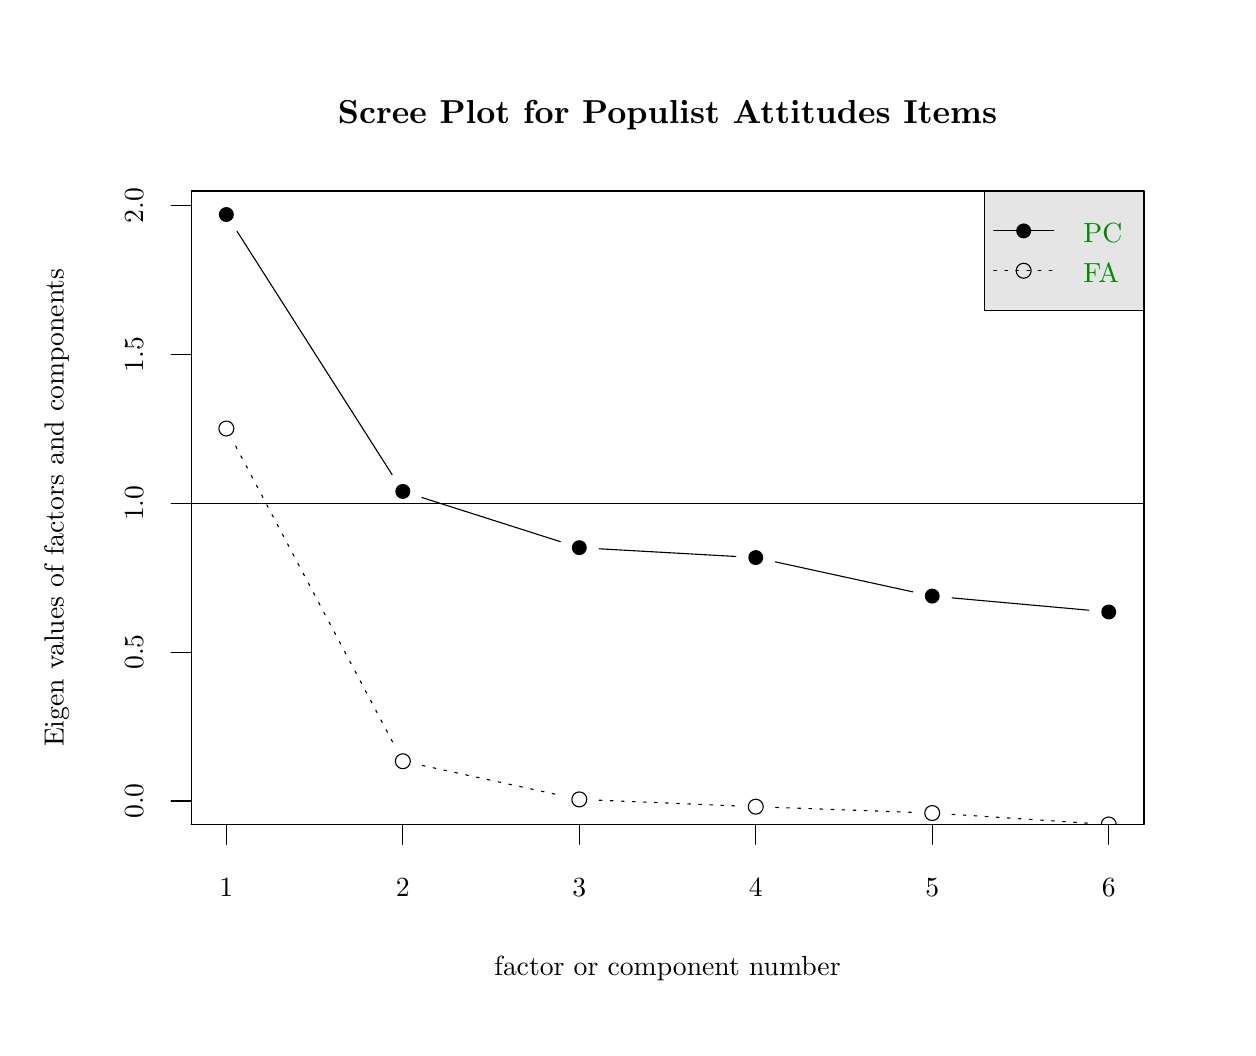
\begin{tikzpicture}[x=1pt,y=1pt]
\definecolor{fillColor}{RGB}{255,255,255}
\path[use as bounding box,fill=fillColor,fill opacity=0.00] (0,0) rectangle (433.62,361.35);
\begin{scope}
\path[clip] ( 59.04, 73.44) rectangle (403.38,302.31);
\definecolor{drawColor}{RGB}{0,0,0}

\path[draw=drawColor,line width= 0.4pt,line join=round,line cap=round] ( 75.66,287.76) -- (131.69,199.84);

\path[draw=drawColor,line width= 0.4pt,line join=round,line cap=round] (142.42,191.58) -- (192.47,175.63);

\path[draw=drawColor,line width= 0.4pt,line join=round,line cap=round] (206.52,173.04) -- (255.90,170.27);

\path[draw=drawColor,line width= 0.4pt,line join=round,line cap=round] (270.13,168.33) -- (319.83,157.48);

\path[draw=drawColor,line width= 0.4pt,line join=round,line cap=round] (334.03,155.30) -- (383.46,150.85);
\definecolor{fillColor}{RGB}{0,0,0}

\path[fill=fillColor] ( 71.79,293.83) circle (  2.70);

\path[fill=fillColor] (135.56,193.77) circle (  2.70);

\path[fill=fillColor] (199.33,173.45) circle (  2.70);

\path[fill=fillColor] (263.09,169.87) circle (  2.70);

\path[fill=fillColor] (326.86,155.95) circle (  2.70);

\path[fill=fillColor] (390.63,150.21) circle (  2.70);
\end{scope}
\begin{scope}
\path[clip] (  0.00,  0.00) rectangle (433.62,361.35);
\definecolor{drawColor}{RGB}{0,0,0}

\path[draw=drawColor,line width= 0.4pt,line join=round,line cap=round] ( 71.79, 73.44) -- (390.63, 73.44);

\path[draw=drawColor,line width= 0.4pt,line join=round,line cap=round] ( 71.79, 73.44) -- ( 71.79, 66.24);

\path[draw=drawColor,line width= 0.4pt,line join=round,line cap=round] (135.56, 73.44) -- (135.56, 66.24);

\path[draw=drawColor,line width= 0.4pt,line join=round,line cap=round] (199.33, 73.44) -- (199.33, 66.24);

\path[draw=drawColor,line width= 0.4pt,line join=round,line cap=round] (263.09, 73.44) -- (263.09, 66.24);

\path[draw=drawColor,line width= 0.4pt,line join=round,line cap=round] (326.86, 73.44) -- (326.86, 66.24);

\path[draw=drawColor,line width= 0.4pt,line join=round,line cap=round] (390.63, 73.44) -- (390.63, 66.24);

\node[text=drawColor,anchor=base,inner sep=0pt, outer sep=0pt, scale=  1.00] at ( 71.79, 47.52) {1};

\node[text=drawColor,anchor=base,inner sep=0pt, outer sep=0pt, scale=  1.00] at (135.56, 47.52) {2};

\node[text=drawColor,anchor=base,inner sep=0pt, outer sep=0pt, scale=  1.00] at (199.33, 47.52) {3};

\node[text=drawColor,anchor=base,inner sep=0pt, outer sep=0pt, scale=  1.00] at (263.09, 47.52) {4};

\node[text=drawColor,anchor=base,inner sep=0pt, outer sep=0pt, scale=  1.00] at (326.86, 47.52) {5};

\node[text=drawColor,anchor=base,inner sep=0pt, outer sep=0pt, scale=  1.00] at (390.63, 47.52) {6};

\path[draw=drawColor,line width= 0.4pt,line join=round,line cap=round] ( 59.04, 81.92) -- ( 59.04,297.10);

\path[draw=drawColor,line width= 0.4pt,line join=round,line cap=round] ( 59.04, 81.92) -- ( 51.84, 81.92);

\path[draw=drawColor,line width= 0.4pt,line join=round,line cap=round] ( 59.04,135.71) -- ( 51.84,135.71);

\path[draw=drawColor,line width= 0.4pt,line join=round,line cap=round] ( 59.04,189.51) -- ( 51.84,189.51);

\path[draw=drawColor,line width= 0.4pt,line join=round,line cap=round] ( 59.04,243.31) -- ( 51.84,243.31);

\path[draw=drawColor,line width= 0.4pt,line join=round,line cap=round] ( 59.04,297.10) -- ( 51.84,297.10);

\node[text=drawColor,rotate= 90.00,anchor=base,inner sep=0pt, outer sep=0pt, scale=  1.00] at ( 41.76, 81.92) {0.0};

\node[text=drawColor,rotate= 90.00,anchor=base,inner sep=0pt, outer sep=0pt, scale=  1.00] at ( 41.76,135.71) {0.5};

\node[text=drawColor,rotate= 90.00,anchor=base,inner sep=0pt, outer sep=0pt, scale=  1.00] at ( 41.76,189.51) {1.0};

\node[text=drawColor,rotate= 90.00,anchor=base,inner sep=0pt, outer sep=0pt, scale=  1.00] at ( 41.76,243.31) {1.5};

\node[text=drawColor,rotate= 90.00,anchor=base,inner sep=0pt, outer sep=0pt, scale=  1.00] at ( 41.76,297.10) {2.0};

\path[draw=drawColor,line width= 0.4pt,line join=round,line cap=round] ( 59.04, 73.44) --
	(403.38, 73.44) --
	(403.38,302.31) --
	( 59.04,302.31) --
	( 59.04, 73.44);
\end{scope}
\begin{scope}
\path[clip] (  0.00,  0.00) rectangle (433.62,361.35);
\definecolor{drawColor}{RGB}{0,0,0}

\node[text=drawColor,anchor=base,inner sep=0pt, outer sep=0pt, scale=  1.20] at (231.21,326.86) {\bfseries Scree Plot for Populist Attitudes Items};

\node[text=drawColor,anchor=base,inner sep=0pt, outer sep=0pt, scale=  1.00] at (231.21, 18.72) {factor or component number};

\node[text=drawColor,rotate= 90.00,anchor=base,inner sep=0pt, outer sep=0pt, scale=  1.00] at ( 12.96,187.87) {Eigen values of factors and components};
\end{scope}
\begin{scope}
\path[clip] ( 59.04, 73.44) rectangle (403.38,302.31);
\definecolor{drawColor}{RGB}{0,0,0}

\path[draw=drawColor,line width= 0.4pt,dash pattern=on 1pt off 3pt ,line join=round,line cap=round] ( 75.17,210.14) -- (132.19,102.64);

\path[draw=drawColor,line width= 0.4pt,dash pattern=on 1pt off 3pt ,line join=round,line cap=round] (142.60, 94.76) -- (192.29, 84.01);

\path[draw=drawColor,line width= 0.4pt,dash pattern=on 1pt off 3pt ,line join=round,line cap=round] (206.52, 82.19) -- (255.90, 80.14);

\path[draw=drawColor,line width= 0.4pt,dash pattern=on 1pt off 3pt ,line join=round,line cap=round] (270.29, 79.59) -- (319.66, 77.82);

\path[draw=drawColor,line width= 0.4pt,dash pattern=on 1pt off 3pt ,line join=round,line cap=round] (334.04, 77.09) -- (383.44, 73.88);

\path[draw=drawColor,line width= 0.4pt,line join=round,line cap=round] ( 71.79,216.50) circle (  2.70);

\path[draw=drawColor,line width= 0.4pt,line join=round,line cap=round] (135.56, 96.28) circle (  2.70);

\path[draw=drawColor,line width= 0.4pt,line join=round,line cap=round] (199.33, 82.48) circle (  2.70);

\path[draw=drawColor,line width= 0.4pt,line join=round,line cap=round] (263.09, 79.85) circle (  2.70);

\path[draw=drawColor,line width= 0.4pt,line join=round,line cap=round] (326.86, 77.56) circle (  2.70);

\path[draw=drawColor,line width= 0.4pt,line join=round,line cap=round] (390.63, 73.42) circle (  2.70);

\path[draw=drawColor,line width= 0.4pt,line join=round,line cap=round] ( 59.04,189.51) -- (403.38,189.51);
\definecolor{fillColor}{gray}{0.90}

\path[draw=drawColor,line width= 0.4pt,line join=round,line cap=round,fill=fillColor] (345.86,302.31) rectangle (403.38,259.11);

\path[draw=drawColor,line width= 0.4pt,line join=round,line cap=round] (349.10,287.91) -- (370.70,287.91);

\path[draw=drawColor,line width= 0.4pt,dash pattern=on 1pt off 3pt ,line join=round,line cap=round] (349.10,273.51) -- (370.70,273.51);
\definecolor{fillColor}{RGB}{0,0,0}

\path[fill=fillColor] (359.90,287.91) circle (  2.70);

\path[draw=drawColor,line width= 0.4pt,line join=round,line cap=round] (359.90,273.51) circle (  2.70);
\definecolor{drawColor}{RGB}{0,139,0}

\node[text=drawColor,anchor=base west,inner sep=0pt, outer sep=0pt, scale=  1.00] at (381.50,283.78) {PC };

\node[text=drawColor,anchor=base west,inner sep=0pt, outer sep=0pt, scale=  1.00] at (381.50,269.38) {FA};
\end{scope}
\end{tikzpicture}
